\section{Alcance}

Definir con precisión el alcance es fundamental para asegurar que el desarrollo se ajuste a los objetivos propuestos y se realice dentro de los recursos y tiempos establecidos. Para ello, en esta sección se delimitarán las funcionalidades, exclusiones y limitaciones que se esperan en este proyecto.

\subsection{Funcionalidades Incluidas}

En la plataforma web se ofrecen las siguientes funcionalidades principales:

\begin{itemize}
    \item \underline{Autenticación segura} mediante las credenciales de \textit{Spotify}.
    \item \underline{\textit{Home} o Panel Inicial} donde se muestran la información básica de la cuenta.
    \item Análisis detallado y visualizaciones \underline{gráficas avanzadas, interactivas y actualizadas} de sus datos musicales.
    \item Interfaz \underline{adaptativa, intuitiva y responsiva}.
    \item \underline{Cierre de sesión seguro}.
\end{itemize}

\subsection{Exclusiones}

Para establecer expectativas claras sobre el alcance del proyecto, se detallan a continuación las funcionalidades que \textbf{no} serán incluidas en la plataforma web:

\begin{itemize}
    \item No se desarrollarán \underline{aplicaciones nativas de otras plataformas} como móvil, PC, Mac o Linux; el acceso será exclusivamente a través de la web.

    \item Aunque se seguirá un diseño intuitivo, no se implementarán funcionalidades específicas de \underline{accesibilidad avanzadas} como compatibilidad con lectores de pantalla o navegación por teclado.

    \item La plataforma se enfoca exclusivamente en la integración con \textit{Spotify}; se excluyen todos los \underline{otros servicios de streaming} como \textit{Apple Music}, \textit{Deezer}, etc.

    \item No se \underline{almacenarán de forma persistente datos personales} del usuario en servidores propios más allá de lo necesario para la sesión actual; todos los datos se obtendrán directamente de la API de \textit{Spotify} y se manejarán en tiempo real.

    \item Se excluye el desarrollo de funcionalidades relacionadas con la \underline{interacción social} (envío de mensajes, compartir estadísticas, rankings entre usuarios, etc.) dentro o a través de la plataforma, ya que superarían el alcance recogido dentro de un TFG.

          % * COMPROBAR SI SE HAN IMPLEMENTADO O NO ESTAS FUNCIONALIDADES * %

          % * \item \textbf{Integración con Redes Sociales}: No se implementarán opciones para compartir estadísticas o visualizaciones directamente en redes sociales como Facebook, Twitter o Instagram.

          % * \item \textbf{Exportación de Datos o Estadísticas}: No se incluirá la opción de exportar los datos o estadísticas a formatos externos como PDF, CSV o imágenes descargables.

          % * \item \textbf{Soporte Multilenguaje}: La interfaz de usuario estará disponible únicamente en español y no se ofrecerá soporte para otros idiomas.

\end{itemize}

\subsection{Limitaciones}

Durante el desarrollo del proyecto, se han identificado las siguientes limitaciones que han afectado al alcance y a las funcionalidades de la web:

\begin{itemize}
    \item Las políticas de seguridad de \textit{Spotify} impiden el \underline{almacenamiento persistente de datos} personales, limitando funcionalidades que requieran conservar información del usuario entre sesiones.

    \item El procesamiento de los datos se ve limitado por los \underline{recursos computacionales} que la nube de \textit{Vercel} ofrece, descartando técnicas avanzadas como el aprendizaje automático.

    \item El \underline{tiempo y los recursos disponibles} para el desarrollo del proyecto son finitos, lo que ha obligado a priorizar funcionalidades esenciales y descartar características adicionales.

    \item Al hacer uso de una API de terceros, todas las funcionalidades necesitan una \underline{conexión} \underline{activa a Internet} para poder funcionar de manera correcta.
\end{itemize}

\section{Gestión de Tareas}

Una vez definido el alcance, es necesario detallar las tareas requeridas para el desarrollo del proyecto. En esta sección se caracterizará todo lo necesario en relación a las tareas, incluyendo su definición, relaciones y tiempos asignados, para asegurar una gestión estructurada y alineada con los objetivos del proyecto.

\subsection{Descripción de Tareas}

Para gestionar de manera efectiva el conjunto de actividades, se ha elaborado una Estructura de Desglose de Trabajo (EDT). Esta EDT (figura \ref{fig:edt}) proporciona una visión general de las principales áreas de trabajo, desglosando el proyecto en paquetes específicos que abarcan cada tarea esencial, facilitando así la gestión.

En este caso, el proyecto se organiza en cinco áreas principales, que abarcan todas las fases del desarrollo de la aplicación; abordando tanto las tareas relacionadas con la creación de la aplicación en sí misma (el producto final) como aquellas enfocadas en la gestión y redacción del proyecto para su documentación. Esta estructura garantiza una distribución clara de las tareas, cubriendo tanto los aspectos técnicos como los organizativos.

\begin{figure}[H]
    \centering
    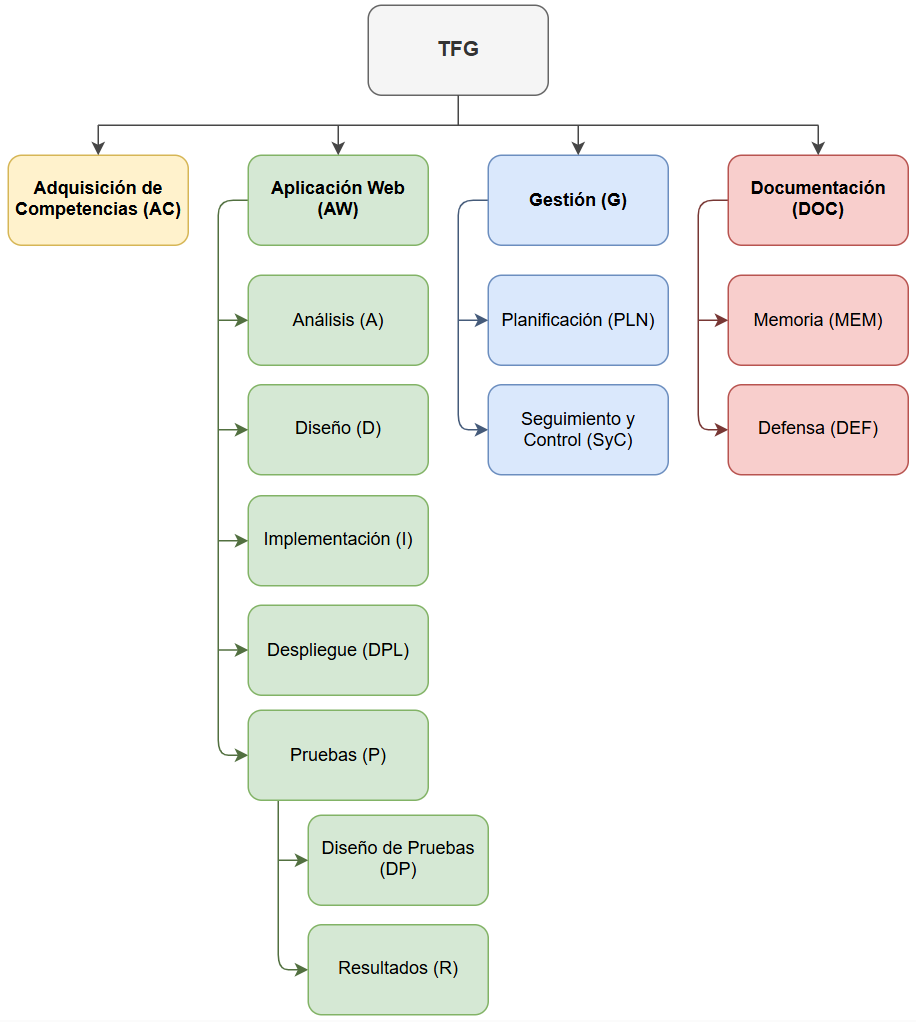
\includegraphics[width=\textwidth]{figures/edt.png}
    \caption{Diagrama EDT con los paquetes de trabajo del proyecto.}
    \label{fig:edt}
\end{figure}

A continuación se detalla cada paquete de trabajo y las tareas correspondientes contenidas en cada una:

\subsubsection{Adquisición de Competencias (AC):}

Este paquete de trabajo incluye todas las tareas necesarias para adquirir el conocimiento sobre las tecnologías y herramientas clave para el desarrollo del proyecto.

\begin{itemize}
    \item \textbf{AC.1:} Aprender \textit{TypeScript}, \textit{React.js} y \textit{Next.js} para el desarrollo de la aplicación web.
    \item \textbf{AC.2:} Estudiar el uso de \textit{Vercel} para el hosting y despliegue de la aplicación.
    \item \textbf{AC.3:} Hacer un reconocimiento inicial de la \textit{Web API} de \textit{Spotify}.
\end{itemize}

\subsubsection{Aplicación Web (AW):}

En este paquete se engloban todas las fases de desarrollo de la aplicación web, desde la planificación inicial hasta el despliegue final.

\begin{itemize}
    \item \textbf{Análisis (A):}
          \begin{itemize}
              \item \textbf{AW.A.1:} Estudiar y analizar en profundidad la \textit{Web API} de \textit{Spotify} para determinar el alcance y sus limitaciones.
              \item \textbf{AW.A.2:} Definir los requisitos funcionales y no funcionales del sistema.
              \item \textbf{AW.A.3:} Desarrollar los principales casos de uso del sistema.
          \end{itemize}

    \item \textbf{Diseño (D):}
          \begin{itemize}
              \item \textbf{AW.D.1:} Diseñar la arquitectura del sistema.
              \item \textbf{AW.D.2:} Crear un diagrama de componentes React para establecer la jerarquía y realizar un diseño general de la interfaz de usuario.
              \item \textbf{AW.D.3:} Definir los diagramas de secuencia de los casos principales.
              \item \textbf{AW.D.4:} Realizar una gestión de la seguridad y asegurar que se implementarán las medidas definidas por \textit{Spotify} para el uso de la API.
          \end{itemize}

    \item \textbf{Implementación (I):}
          \begin{itemize}
              \item \textbf{AW.I.1:} Implementar el login de la página web, usando el protocolo OAuth 2.0 implementado por \textit{Spotify}.
              \item \textbf{AW.I.2:} Implementar el panel inicial (dashboard) de la web.
              \item \textbf{AW.I.3:} Implementar la sección principal de estadísiticas.
              \item \textbf{AW.I.4:} Implementar la funcionalidad de cerrar sesión.
              \item \textbf{AW.I.5:} Realizar optimizaciones y correcciones en la implementación.
          \end{itemize}

    \item \textbf{Despliegue (DPL):}
          \begin{itemize}
              \item \textbf{AW.DPL.1:} Configurar el despliegue en \textit{Vercel} para crear un proceso automático de despliegue.
              \item \textbf{AW.DPL.2:} Monitorear el funcionamiento del despliegue y los logs.
          \end{itemize}
\end{itemize}

\subsubsection{Pruebas (P):}

Este paquete agrupa las tareas relacionadas con la verificación y validación de la aplicación, garantizando su correcto funcionamiento y calidad.

\begin{itemize}
    \item \textbf{Diseño de Pruebas (DP):} Planificar y diseñar pruebas unitarias, de integración y de carga para evaluar el rendimiento y la estabilidad de la aplicación.
    \item \textbf{Resultados (R):}
          \begin{itemize}
              \item \textbf{P.R.1:} Realizar las pruebas planificadas y documentar los errores encontrados.
              \item \textbf{P.R.2:} Definir y, en caso de que sea posible, implementar las correcciones necesarias.
          \end{itemize}
\end{itemize}

\subsubsection{Gestión (G):}

\begin{itemize}
    \item \textbf{Planificación (PLN):}
          \begin{itemize}
              \item \textbf{G.PLN.1:} Realizar una primera estimación de tiempos de las tareas generales.
              \item \textbf{G.PLN.2:} Establecer el alcance inicial del proyecto según las características del producto seleccionadas.
              \item \textbf{G.PLN.3:} Definir la planificación del proyecto.
              \item \textbf{G.PLN.4:} Revisar y, si fuera necesario, modificar la planificación.
          \end{itemize}
    \item \textbf{Seguimiento y Control (SyC):}
          \begin{itemize}
              \item \textbf{G.SyC.1:} Conversaciones y comentarios de la tutora a lo largo del desarrollo.
              \item \textbf{G.SyC.2:} Elaboración de un documento para registrar las actividades y dedicaciones realizadas a lo largo del proyecto.
              \item \textbf{G.SyC.3:} Comparación de los datos del seguimiento con los de la placificación, identificación de las desviaciones y riesgos significativos.
          \end{itemize}
\end{itemize}

\subsubsection{Documentación (DOC):}

Este paquete agrupa las tareas necesarias para la elaboración de la memoria y la preparación de la defensa del proyecto.

\begin{itemize}
    \item \textbf{Memoria (MEM):}
          \begin{itemize}
              \item \textbf{DOC.MEM.1:} Preparar el entorno de trabajo en \LaTeX\ utilizando \textit{Visual Studio Code} y establecer la estructura básica de la memoria a partir de la plantilla proporcionada por la facultad.
              \item \textbf{DOC.MEM.2:} Redactar la memoria.
          \end{itemize}
    \item \textbf{Defensa (DEF):}
          \begin{itemize}
              \item \textbf{DOC.DEF.1:} Identificar los puntos y conceptos clave que se presentarán en la defensa.
              \item \textbf{DOC.DEF.2:} Crear los elementos visuales de apoyo para la defensa.
              \item \textbf{DOC.DEF.3:} Preparar y ensayar la defensa.
          \end{itemize}
\end{itemize}

\cleardoublepage

\subsection{Dedicaciones}

A continuación, en la tabla \ref{tab:estimaciones_tareas}, se presentan las horas estimadas para las tareas descritas en el apartado anterior. También se muestran las sumas de las dedicaciones por paquete de trabajo y la suma total de horas que se espera que lleve el desarrollo del proyecto completo.

\begin{table}[H]
    \centering
    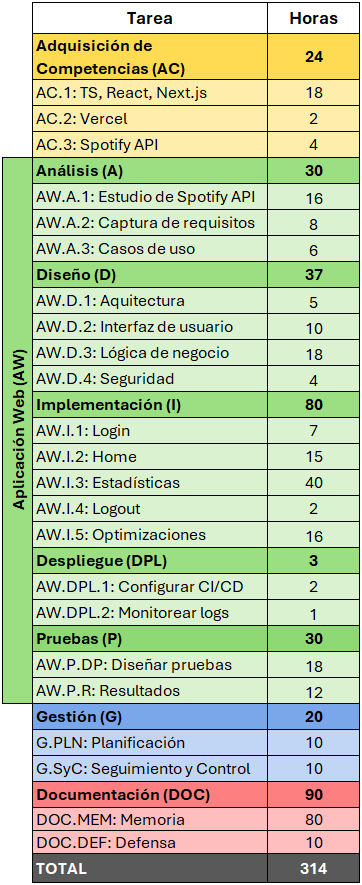
\includegraphics[width=0.55\textwidth]{figures/estimaciones_tareas.png}
    \caption{Tabla con las estimaciones de tiempo por paquete de trabajo y tarea del proyecto.}
    \label{tab:estimaciones_tareas}
\end{table}

\subsection{Dependencias entre Tareas}

En la figura \ref{fig:dependencias_tareas} se muestra un diagrama representando las dependencias que existen entre las diferentes tareas. De esta manera, se puede apreciar de forma visual las tareas que requieren la finalización de una o varias tareas para su comiezo.

\begin{figure}[H]
    \centering
    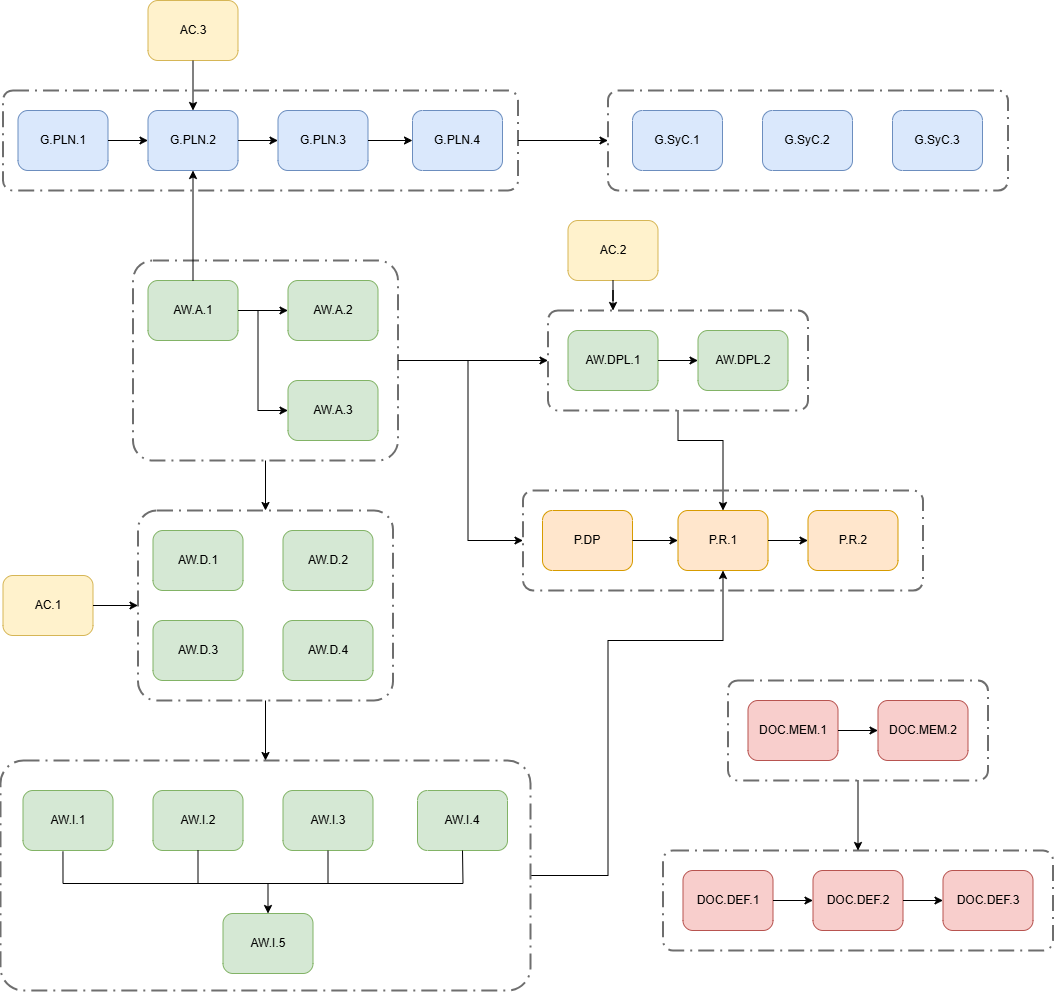
\includegraphics[width=\textwidth]{figures/dependencias_tareas.png}
    \caption{Diagrama de dependencias entre las tareas y paquetes de trabajo del proyecto.}
    \label{fig:dependencias_tareas}
\end{figure}

Como se puede apreciar, el proyecto debe iniciarse con las tareas de la planificación (paquete de trabajo \textbf{G.PLN}) y análisis (\textbf{AW.A}), al igual que el desarrollo de las tareas relacionadas con la memoria (\textbf{DOC.MEM}), que se realizan desde el inicio del proyecto hasta casi la finalización del TFG. Para ordenar temporalmente todas las tareas, en la siguiente sección se tratarán los periodos de desarrollo de cada una.

\newpage

\subsection{Periodos de Desarrollo e Hitos}

En esta sección se presenta el diagrama Gantt del proyecto (figura \ref{fig:gantt}), el cual ilustra los periodos de realización de las tareas y los paquetes de trabajo; siempre teniendo en cuenta las dedicaciones asignadas y las dependencias entre las tareas que se han establecido en la sección anterior. Además, se destacan los hitos del proyecto, permitiendo una visualización clara y organizada del cronograma planificado.

\begin{figure}[H]
    \centering
    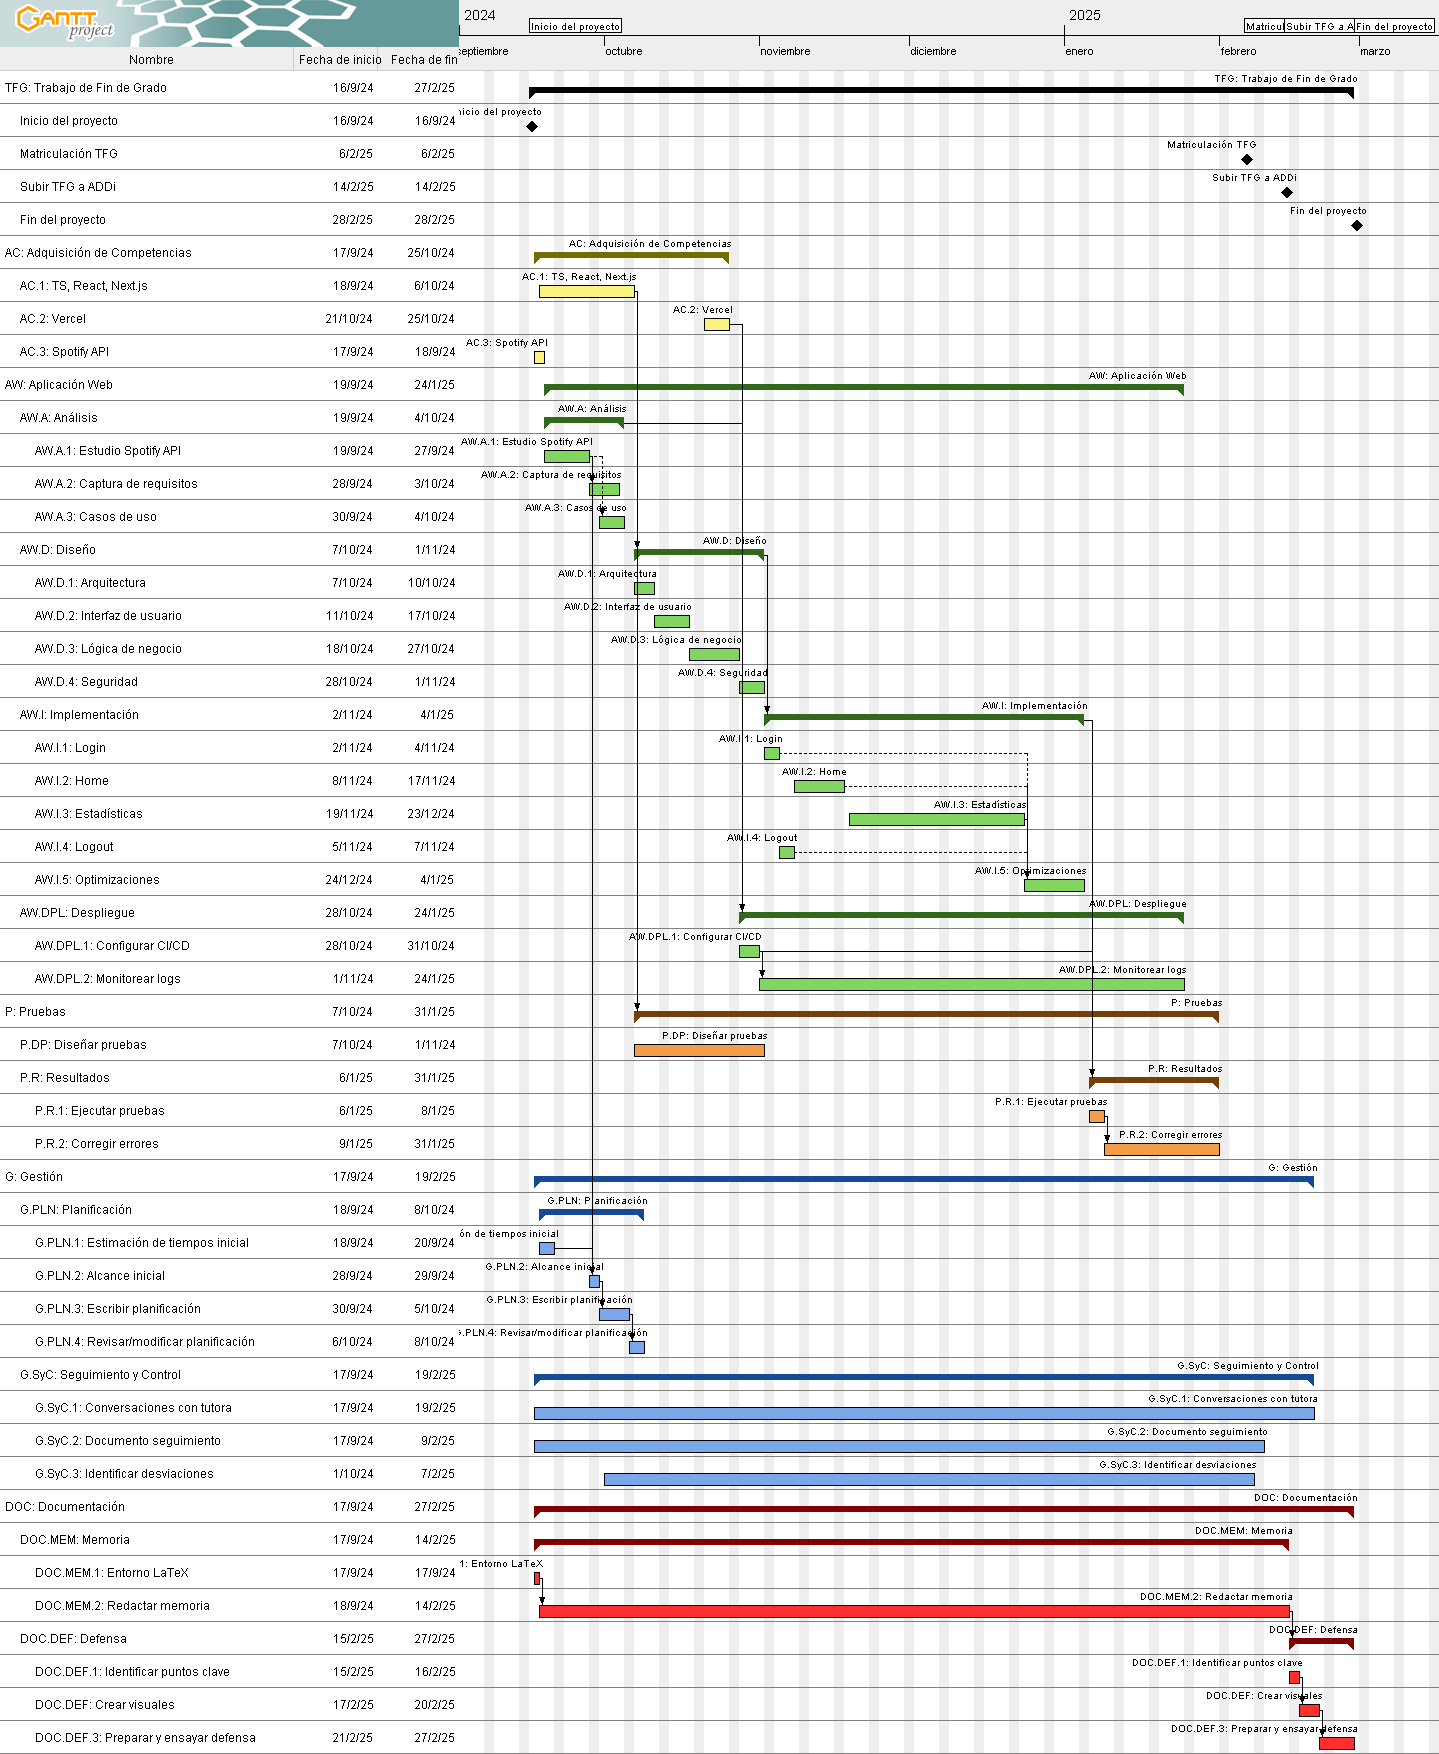
\includegraphics[width=\textwidth]{figures/gantt.png}
    \caption{Diagrama Gantt con los tiempos de realización de las tareas y paquetes de trabajo.}
    \label{fig:gantt}
\end{figure}

\section{Gestión de Riesgos}

La gestión de riesgos desempeña un papel crucial en cualquier proyecto, ya que permite anticiparse a posibles inconvenientes, definiendo estrategias adecuadas para minimizar su impacto sobre el proyecto.

A continuación, se presentan los riesgos identificados, especificando para cada uno de ellos la probabilidad de que se materialice, el impacto que podría ocasionar, las medidas implementadas para prevenirlos y las acciones que se llevarían a cabo en caso de que se acabe materializando alguno de ellos.

\subsection{R01: Limitaciones con respecto a los datos disponibles de la API}
Este riesgo se refiere a la posible falta de datos suficientes o adecuados para implementar ciertas funcionalidades previstas, como estadísticas o visualizaciones concretas.

\begin{itemize}
    \item \textbf{Probabilidad}: Media.
    \item \textbf{Impacto}: Medio.
    \item \textbf{Prevención}: Analizar detenidamente los endpoints de la API antes de planificar funcionalidades dependientes de datos específicos.
    \item \textbf{Plan de mitigación}: Proponer gráficos o funcionalidades alternativas que no dependan de esos datos.
\end{itemize}

\subsection{R02: Cambios en la política de acceso a la API}
Como \textit{Spotify} se reserva el derecho de modificar en cualquier momento las políticas de uso de su API, existe la posibilidad de que algunas funcionalidades del proyecto se vean afectadas o limitadas debido a cambios en los permisos o en la disponibilidad de ciertos endpoints.

\begin{itemize}
    \item \textbf{Probabilidad}: Baja.
    \item \textbf{Impacto}: Alto.
    \item \textbf{Prevención}: Revisar con frecuencia la documentación oficial y adaptar el proyecto a los permisos disponibles desde el inicio.
    \item \textbf{Plan de mitigación}: Ajustar el alcance del proyecto para trabajar con los datos que sigan siendo accesibles y documentar los cambios en la memoria del TFG.
\end{itemize}

\subsection{R03: Interrupciones en la disponibilidad de servicios de terceros}
Este riesgo engloba posibles problemas de disponibilidad en servicios externos críticos para el proyecto, como la API de \textit{Spotify} o el servicio de hosting de \textit{Vercel}.

\begin{itemize}
    \item \textbf{Probabilidad}: Baja.
    \item \textbf{Impacto}: Alto.
    \item \textbf{Prevención}: Mantener una planificación que contemple margen suficiente para posibles retrasos causados por la indisponibilidad de estos servicios. Además, probar despliegues en un entorno local para avanzar en el desarrollo mientras el servicio de hosting se restablece.
    \item \textbf{Plan de mitigación}: Continuar con el desarrollo de los aspectos que no dependan de estos servicios y retomar las tareas una vez se solucione la interrupción.
\end{itemize}

\subsection{R04: Incompatibilidad de versiones de las tecnologías a utilizar}
Este riesgo está relacionado con posibles problemas de compatibilidad entre \textit{TypeScript}, \textit{React}, \textit{Next.js} y las librerías utilizadas.

\begin{itemize}
    \item \textbf{Probabilidad}: Media.
    \item \textbf{Impacto}: Alto.
    \item \textbf{Prevención}: Investigar y verificar compatibilidades antes de seleccionar versiones específicas. Evitar usar, en la medida de lo posible, versiones muy recientes que puedan tener problemas de estabilidad y de soporte por parte de otras herramientas.
    \item \textbf{Plan de mitigación}: Actualizar o cambiar las herramientas o librerías problemáticas por alternativas compatibles y realizar pruebas exhaustivas después de cada cambio.
\end{itemize}

\subsection{R05: Dificultad en el aprendizaje de las herramientas a utilizar}
Al trabajar con herramientas, frameworks y tecnologías con los que no se ha tenido un contacto previo, se pueden ocasionar retrasos por el proceso de aprendizaje.

\begin{itemize}
    \item \textbf{Probabilidad}: Media.
    \item \textbf{Impacto}: Medio.
    \item \textbf{Prevención}: Reservar un tiempo de adquisición de conocimientos y realizar pruebas antes de comenzar con las implementaciones críticas.
    \item \textbf{Plan de mitigación}: Consultar documentación oficial, foros o buscar ayuda en comunidades de desarrollo en línea para resolver dudas rápidamente. Si no es suficiente, se puede avanzar con otra tarea que no dependa de la resolución del problema actual, permitiendo ganar tiempo mientras se sigue investigando la solución al inconveniente técnico.
\end{itemize}

\subsection{R06: Planificación incorrecta}
Como puede ocurrir en cualquier proyecto, este riesgo consiste en una planificación inicial que no contemple adecuadamente el tiempo o los recursos necesarios para el desarrollo del proyecto.

\begin{itemize}
    \item \textbf{Probabilidad}: Media.
    \item \textbf{Impacto}: Alto.
    \item \textbf{Prevención}: Elaborar una planificación con plazos amplios y flexibles que permita realizar ajustes sin comprometer la entrega final.
    \item \textbf{Plan de mitigación}: Reorganizar tareas y replantear las prioridades para cumplir los objetivos principales y siempre minimizando el impacto.
\end{itemize}

\subsection{R07: Dificultad para compaginar el proyecto con las obligaciones académicas}
Este riesgo hace referencia a la posibilidad de tener problemas a la hora de gestionar el tiempo disponible para dedicar al proyecto, ya que se está cursando una asignatura en paralelo.

\begin{itemize}
    \item \textbf{Probabilidad}: Media.
    \item \textbf{Impacto}: Alto.
    \item \textbf{Prevención}: Planificar un calendario detallado y realista que reserve horas específicas para trabajar en el proyecto, priorizando las tareas críticas.
    \item \textbf{Plan de mitigación}: Ajustar la planificación redistribuyendo tareas menos prioritarias y minimizando así el impacto en el desarrollo del proyecto.
\end{itemize}

% * He decidido no hacer la Gestión de Calidad
% \section{Gestión de Calidad}

\section{Herramientas y Tecnologías}
